% Documento autónomo en UTF-8, legible como texto plano.
% Conversión de la propuesta original; no agrega resultados empíricos.
% Contiene ecuaciones, pseudocódigo, tablas, figura vectorial y bibliografía.
% Compilación opcional: pdflatex (dos pasadas). No necesita .bib ni imágenes.
\documentclass[11pt,letterpaper]{article}
\usepackage[utf8]{inputenc}
\usepackage[T1]{fontenc}
\renewcommand{\refname}{Referencias}
\renewcommand{\figurename}{Figura}
\usepackage[margin=2.2cm]{geometry}
\usepackage{lmodern}
\usepackage{amsmath,amssymb}
\usepackage{longtable,booktabs,array,calc}
\usepackage{xurl}
\usepackage[hidelinks]{hyperref}
\usepackage{pgfplots}
\pgfplotsset{compat=1.18}
\usepgfplotslibrary{fillbetween}
\setlength{\parindent}{0pt}
\setlength{\parskip}{6pt}
\setlength{\emergencystretch}{3em}
\title{Selección de variables para scorecards mediante búsqueda evolutiva con restricciones\\[6pt]\large Propuesta metodológica y protocolo experimental}
\author{}
\date{22 de septiembre de 2026}
\begin{document}
\maketitle

\section*{Resumen}

Se propone desarrollar un algoritmo de selección de variables para scorecards logísticas que maximice el AUC promedio de validación cruzada bajo restricciones de cardinalidad, familias económicas, incompatibilidades, information value y multicolinealidad. La unidad de búsqueda será un conjunto completo de variables; la unidad de evaluación, el entrenamiento y validación de ese conjunto mediante un procedimiento fijo y reproducible. El algoritmo combinará una población genética, intercambios locales, propuestas aleatorias y un modelo sustituto que priorice qué candidatos merecen una evaluación completa. Se denomina provisionalmente SEF, selector evolutivo por familias.

La decisión metodológica principal es conservar el AUC de CV como objetivo primario, en vez de mezclar desde el inicio discriminación, estabilidad y complejidad en una suma con ponderaciones arbitrarias. La estabilidad temporal, la calibración y la variación de la selección se medirán explícitamente. Para la elección operacional se propondrá una regla de preferencia entre soluciones cercanas en AUC, separada del objetivo utilizado para comparar optimizadores.

El estudio propuesto distinguirá eficiencia de búsqueda y generalización. En problemas pequeños se enumerará el espacio factible para construir un oráculo exhaustivo y medir la brecha al óptimo frente al número de ensayos. En problemas grandes se compararán métodos con el mismo presupuesto, sin llamar óptimo a la mejor solución observada. Se incluirán búsqueda aleatoria, forward, stepwise, búsqueda local, un genético sin asistencia y TPE. La evaluación predictiva requerirá validación externa al proceso completo de selección y, cuando existan datos longitudinales, pruebas temporales que respeten la disponibilidad de etiquetas.

Este documento es una propuesta. No se han implementado los algoritmos, entrenado modelos ni producido resultados experimentales. Los parámetros son decisiones iniciales que deberán preregistrarse o ajustarse exclusivamente en tareas de desarrollo separadas. La figura incluida es un esquema ilustrativo, no evidencia de superioridad.

\textbf{Palabras clave:} scorecard, selección de variables, restricciones de negocio, algoritmo genético, AUC, optimización combinatoria, validación temporal.

\section{Problema de investigación}\label{sec:1}

La selección de variables de una scorecard no consiste solamente en identificar predictores con asociación marginal al incumplimiento. Debe encontrar una combinación que aporte discriminación conjunta, mantenga una interpretación económica coherente y satisfaga condiciones de implementación y validación. Por ejemplo, máximo de mora en tres meses y máximo de mora en seis meses pueden competir por representar un mismo concepto aunque ambas variables tengan alto IV.

El stepwise modifica un conjunto mediante decisiones locales. Una sustitución beneficiosa puede exigir retirar dos variables e incorporar otras dos, atravesando una solución intermedia de menor desempeño. Una búsqueda exhaustiva resuelve la comparación dentro de un espacio finito definido, pero su costo crece rápidamente. La propuesta busca una alternativa intermedia: explorar de manera adaptativa sin enumerar todos los subconjuntos y conservar trazabilidad de cada decisión.

La pregunta principal será: ¿puede un buscador especializado en familias e incompatibilidades alcanzar una solución cercana al mejor AUC de CV factible con menos evaluaciones que los métodos de referencia, sin deteriorar la generalización ni la estabilidad del procedimiento de selección?

No se supone que exista una combinación universalmente mejor. El resultado depende de los datos, la definición del objetivo, el binning, las restricciones y la regla de validación. Tampoco se presupone que una heurística encuentre el óptimo global.

\subsection{Contribución que se pretende evaluar}\label{sec:1.1}

La contribución propuesta es la integración verificable de cuatro componentes: representación explícita de sustituciones económicas; generación y reparación de candidatos factibles; aprendizaje del desempeño de conjuntos completos; y evaluación contra un oráculo exhaustivo aislado del optimizador. Cada componente tendrá una ablación para determinar si aporta valor por separado.

La selección genética con conocimiento experto y la asistencia mediante aproximaciones ya tienen antecedentes. Por lo tanto, no se reivindica haber inventado esas ideas. Una eventual contribución científica requerirá demostrar que la arquitectura específica para scorecards mejora el compromiso entre costo de búsqueda, discriminación y estabilidad bajo restricciones realistas.

\section{Antecedentes y decisiones derivadas}\label{sec:2}

Lappas y Yannacopoulos \cite{ref1} proponen combinar conocimiento experto y algoritmos genéticos para selección de variables en riesgo crediticio. Este antecedente justifica investigar una representación que incorpore reglas de negocio. No constituye evidencia de que la arquitectura aquí propuesta supere a otros métodos, ni de que sus resultados se transfieran a una scorecard WOE logística. El alcance revisado de este trabajo corresponde a la información pública de la publicación.

BOCS \cite{ref2} estudia optimización de funciones costosas sobre estructuras combinatorias. CASMOPOLITAN \cite{ref3} combina búsqueda local y modelos para espacios categóricos y mixtos. Ambos muestran líneas relevantes para aprender sobre combinaciones, pero su adaptación a cardinalidad exacta, familias e incompatibilidades exige diseño adicional.

SAGA \cite{ref4} y el trabajo sobre aproximaciones cualitativas de algoritmos genéticos \cite{ref5} estudian cómo reducir el costo de selección wrapper. Estos antecedentes motivan priorizar evaluaciones mediante información aproximada. En nuestra propuesta, el sustituto predecirá el AUC del conjunto a partir de evaluaciones anteriores; no se asumirá que reproducimos los mecanismos concretos de esas publicaciones.

Cawley y Talbot \cite{ref6} muestran que optimizar un criterio estimado puede sobreajustar el propio proceso de selección. Esta observación exige evaluar el procedimiento completo fuera de los datos utilizados para buscar. Nogueira, Sechidis y Brown \cite{ref7} proporcionan una base para medir estabilidad de selección; adoptaremos esa perspectiva sin equiparar repetibilidad entre semillas con estabilidad frente a cambios de muestra.

Deb \cite{ref8} ofrece un antecedente para tratar factibilidad sin depender exclusivamente de penalizaciones arbitrarias. La propuesta utiliza restricciones duras y estados explícitos de rechazo. El trabajo clásico sobre AUC de Hanley y McNeil \cite{ref9} fundamenta su interpretación como medida de ordenamiento.

\begin{longtable}[]{@{}
  >{\raggedright\arraybackslash}p{(\columnwidth - 4\tabcolsep) * \real{0.3333}}
  >{\raggedright\arraybackslash}p{(\columnwidth - 4\tabcolsep) * \real{0.3333}}
  >{\raggedright\arraybackslash}p{(\columnwidth - 4\tabcolsep) * \real{0.3333}}@{}}
\toprule\noalign{}
\begin{minipage}[b]{\linewidth}\raggedright
Antecedente
\end{minipage} & \begin{minipage}[b]{\linewidth}\raggedright
Uso en la propuesta
\end{minipage} & \begin{minipage}[b]{\linewidth}\raggedright
Lo que no se transfiere automáticamente
\end{minipage} \\
\midrule\noalign{}
\endhead
\bottomrule\noalign{}
\endlastfoot
Genéticos con conocimiento experto \cite{ref1} & Familias y reglas económicas & Superioridad en WOE logística \\
BOCS y CASMOPOLITAN \cite{ref2,ref3} & Aprendizaje sobre combinaciones & Garantías para nuestro espacio restringido \\
SAGA y aproximaciones cualitativas \cite{ref4,ref5} & Reducir evaluaciones costosas & Aceleraciones publicadas en otros problemas \\
Sesgo de selección \cite{ref6} & Evaluación anidada y OOT reservado & Corrección por usar CV una sola vez \\
Estabilidad de selección \cite{ref7} & Comparación por muestra y familia & Inferencia válida usando semillas como muestras \\
Manejo de restricciones \cite{ref8} & Factibilidad antes que desempeño & Certificar factibilidad estadística sin calcularla \\
\end{longtable}

\section{Formulación del espacio de búsqueda}\label{sec:3}

Sean \(p\) variables candidatas y \(S\) el subconjunto seleccionado. Definimos \(z_j=1\) cuando la variable \(j\) pertenece a \(S\) y \(z_j=0\) en caso contrario. Inicialmente se buscarán exactamente \(k=6\) variables. Posteriormente se podrá repetir el protocolo para distintos tamaños; el tamaño no se elegirá usando el test final.

Las familias serán conjuntos disjuntos \(F_1,\ldots,F_G\) de variables consideradas sustitutos cercanos. Es conveniente distinguir familia de sustitución de dominio económico. Máximo de mora a distintas ventanas puede constituir una familia; nivel, recurrencia y tendencia de mora podrían pertenecer a familias distintas dentro del dominio morosidad, si el criterio de negocio permite su coexistencia.

Una regla demasiado amplia, como permitir una única variable de toda la morosidad, puede excluir combinaciones útiles por definición. El catálogo de familias debe aprobarse antes de comparar resultados. Se admitirán grupos adicionales solapados e incompatibilidades entre variables de familias diferentes.

Las restricciones estructurales principales serán:

\[
z_j\in\{0,1\},\qquad \sum_{j=1}^{p}z_j=k,\qquad
\sum_{j\in F_g}z_j\leq 1\quad \forall g.
\]

Si \(E\) contiene pares incompatibles, se añadirá:

\[
z_i+z_j\leq 1\quad \forall (i,j)\in E.
\]

Variables obligatorias y prohibidas se expresarán mediante valores fijos de \(z_j\). Las cuotas por origen o dominio se representarán como límites inferiores y superiores sobre sumas de indicadores. Por ejemplo, una cuota de variables internas y externas es una regla adicional, no una consecuencia de las familias.

\subsection{Tamaño del espacio antes de filtros estadísticos}\label{sec:3.1}

Si la familia \(g\) contiene \(n_g\) variables, la cantidad de subconjuntos con exactamente \(k\) variables y máximo una por familia es el coeficiente de grado \(k\) del producto:

\[
N_k=[x^k]\prod_{g=1}^{G}(1+n_gx).
\]

Cada factor representa no elegir esa familia, con contribución 1, o elegir una de sus variables, con contribución \(n_gx\). Al multiplicar, los términos de grado \(k\) cuentan elecciones de exactamente \(k\) familias. Si todas tienen \(m\) variables, primero se eligen \(k\) familias y luego una de las \(m\) variables de cada una:

\[
N_k=\binom{G}{k}m^k.
\]

Para seis familias con cinco variables y seis seleccionadas, \(N_6=5^6=15\,625\). Si fueran doce familias con cinco variables y se eligieran seis, \(N_6=\binom{12}{6}5^6=14\,437\,500\). Estas cifras no incorporan incompatibilidades, IV, correlación ni VIF; son cotas superiores del espacio finalmente admisible.

La restricción de máximo una variable por familia, por sí sola, tiene estructura de matroide de partición. Al agregar incompatibilidades y restricciones estadísticas no se asume que la región completa conserve esa estructura ni que el AUC sea submodular. Por eso no se invocarán garantías de optimalidad de un algoritmo greedy.

\section{Objetivo de optimización y modelo predictivo}\label{sec:4}

\subsection{Por qué AUC como objetivo principal}\label{sec:4.1}

Se propone maximizar el promedio de AUC en particiones de validación fijas. El AUC evalúa el ordenamiento global de casos positivos frente a negativos y no requiere seleccionar un umbral. KS identifica la mayor separación entre distribuciones y puede ser sensible a dónde aparece ese máximo. Esta diferencia motiva preferir AUC, pero no demuestra que su varianza sea siempre menor. Esa hipótesis se contrastará con remuestreo y comparaciones de ranking de candidatos.

Para un fold con \(n_+\) incumplidores y \(n_-\) no incumplidores, orientando el score hacia mayor riesgo:

\[
\widehat{AUC}=\frac{1}{n_+n_-}\sum_{i:y_i=1}\sum_{j:y_j=0}
\left[\mathbf{1}(s_i>s_j)+\frac{1}{2}\mathbf{1}(s_i=s_j)\right].
\]

La media de comparaciones asigna un punto a cada pareja correctamente ordenada y medio punto a un empate. Esta definición hace explícito el tratamiento de empates de las scorecards. Si el puntaje operacional aumenta con la calidad crediticia, se invertirá su orientación para calcular AUC.

Con \(K\) folds válidos, el objetivo será:

\[
J(S)=\frac{1}{K}\sum_{r=1}^{K}\widehat{AUC}_r(S),\qquad
S^*\in\underset{S\in\mathcal{F}}{\arg\max}\ J(S).
\]

La media dará el mismo peso a cada fold. Para validación temporal, se elegirán ventanas de duración comparable; cualquier ponderación distinta se fijará antes de buscar. No se sustituirá automáticamente esta media por el AUC de todas las predicciones out of fold concatenadas: este último incorpora comparaciones entre observaciones puntuadas por modelos distintos.

Todos los candidatos usarán los mismos folds y semillas del evaluador. Así, la trayectoria de búsqueda refleja principalmente qué combinaciones se prueban, en vez de cambiar simultáneamente el candidato y su partición. Esta decisión reduce una fuente de ruido comparativo, pero no elimina el error muestral ni el sobreajuste a CV.

\subsection{Qué queda fuera de la función objetivo}\label{sec:4.2}

KS, PR-AUC, log loss, Brier, calibración, AUC por período y PSI se registrarán como diagnósticos. Maximizar AUC no garantiza probabilidades bien calibradas ni optimiza por sí solo rentabilidad, provisiones o una región particular de la curva ROC. El Gini normalizado habitual, calculado como \(2AUC-1\), induce el mismo orden de candidatos y no aporta otro objetivo independiente.

No se incorporará inicialmente una penalización del tipo media menos una constante por desviación entre folds. La dispersión puede reflejar cambios genuinos entre poblaciones o períodos, y no es un error estándar de la media. Introducir esa penalización añade otra decisión de modelamiento y cambia el óptimo con el que se comparan los algoritmos.

\subsection{Especificación de la scorecard evaluada}\label{sec:4.3}

La versión principal usará binning univariado, transformación WOE y regresión logística aditiva. Cada variable seleccionada aportará un coeficiente WOE; no se agregarán interacciones en el clasificador durante este estudio. Las interacciones del sustituto se referirán al desempeño de combinaciones de variables, no a nuevos términos de la scorecard.

Se fijará la convención \(WOE=\log(p_{bad}/p_{good})\). Las proporciones se calcularán en entrenamiento con suavizado y reglas de bins predefinidos. La probabilidad tendrá la forma:

\[
\Pr(Y=1\mid X,S)=\sigma\left(\beta_0+\sum_{j\in S}\beta_jWOE_j(X_j)\right),
\qquad \sigma(u)=\frac{1}{1+e^{-u}}.
\]

Para mantener el ajuste inicial cercano a una scorecard convencional, se utilizará máxima verosimilitud sin regularización. Se rechazarán candidatos con falta de convergencia, estimaciones no finitas, separación detectada o coeficientes con signo contrario a la convención, según tolerancias numéricas fijas. Esta regla también se aplicará a los comparadores de espacio común. No se cambiará de estimador silenciosamente para rescatar un candidato.

Una variante separada estudiará logística con regularización L2 fija o restricciones de signo en el ajuste. Su evaluación exhaustiva y sus referencias deberán recalcularse porque modifica la función objetivo. No se optimizarán simultáneamente binning, regularización y selección en el primer experimento: interesa aislar el aporte del buscador.

\section{Restricciones estadísticas y tratamiento de factibilidad}\label{sec:5}

Las restricciones se verificarán sobre la representación que entra a la logística, usando solamente el entrenamiento de cada fold para ajustar WOE y calcular estadísticas. La elegibilidad conjunta para la búsqueda podrá exigir que se cumplan en todos los folds. Esta intersección forma parte del selector interno; no convierte el AUC de CV en una estimación externa independiente.

\begin{longtable}[]{@{}
  >{\raggedright\arraybackslash}p{(\columnwidth - 4\tabcolsep) * \real{0.3333}}
  >{\raggedright\arraybackslash}p{(\columnwidth - 4\tabcolsep) * \real{0.3333}}
  >{\raggedright\arraybackslash}p{(\columnwidth - 4\tabcolsep) * \real{0.3333}}@{}}
\toprule\noalign{}
\begin{minipage}[b]{\linewidth}\raggedright
Condición
\end{minipage} & \begin{minipage}[b]{\linewidth}\raggedright
Regla inicial
\end{minipage} & \begin{minipage}[b]{\linewidth}\raggedright
Momento de evaluación
\end{minipage} \\
\midrule\noalign{}
\endhead
\bottomrule\noalign{}
\endlastfoot
Cardinalidad & Exactamente seis variables & Generación y reparación \\
Familia & Máximo una por familia & Generación y reparación \\
Incompatibilidad conceptual & Ningún par prohibido & Antes de ajustar modelos \\
IV & Mayor que 0,1 en cada entrenamiento & Precomputación por fold \\
Correlación & Absoluta menor que 0,7 en cada entrenamiento & Grafo de conflictos \\
VIF & Menor que 5 para cada variable y fold & Candidato completo \\
Ajuste logístico & Convergencia y coeficientes admisibles & Entrenamiento por fold \\
\end{longtable}

Los umbrales anteriores reproducen una configuración de estudio; no son umbrales universales ni exigencias regulatorias. Exigir IV mayor que 0,1 puede descartar variables con poco aporte marginal y buen aporte condicional. Se mantendrá como restricción solicitada en el experimento principal y se analizará su costo en escenarios alternativos fijados previamente.

\subsection{IV y correlación}\label{sec:5.1}

El IV se calculará a partir de los mismos bins de entrenamiento y la misma convención de WOE. Bins de nulos, códigos especiales, categorías nuevas y suavizado tendrán una política común. Ninguna estadística supervisada se calculará sobre toda la muestra antes de separar entrenamiento y validación.

La correlación principal será Pearson sobre WOE. Así se controla dependencia lineal entre los regresores efectivos. La correlación de variables originales y Spearman servirán de diagnóstico conceptual, sin reemplazar las incompatibilidades de negocio. Una pareja se prohibirá si infringe el límite en cualquiera de los entrenamientos internos. Una variable constante se declarará inadmisible, en lugar de convertir una correlación indefinida en cero.

\subsection{VIF como condición del conjunto completo}\label{sec:5.2}

Para cada variable seleccionada se ajustará una regresión auxiliar con intercepto contra las demás variables del conjunto. Con su coeficiente de determinación:

\[
VIF_j(S)=\frac{1}{1-R_j^2(S)}.
\]

Cuando la matriz de correlaciones \(R_S\) es invertible, los VIF corresponden a su diagonal inversa. Podrán obtenerse mediante soluciones de sistemas lineales, evitando una inversión numérica innecesaria. Una singularidad implicará rechazo. No se usará una pseudoinversa para declarar aceptable una dependencia exacta.

Correlaciones moderadas de a pares no garantizan VIF bajo: una variable puede aproximarse mediante una combinación de varias otras. Por eso el VIF se comprueba después del filtro por pares, aunque ambos controles parezcan relacionados.

\subsection{Reparación y ausencia de soluciones}\label{sec:5.3}

El grafo de conflictos tendrá variables como nodos y pares incompatibles como aristas. La reparación estructural buscará un conjunto de tamaño \(k\) compatible, conservando tantas elecciones parentales como sea posible. Se propone usar un pequeño problema binario con objetivo de mínima distancia respecto del candidato original; desempates aleatorios con semilla impedirán devolver siempre la misma reparación.

La reparación solo certificará reglas estructurales y conflictos precalculados. El VIF y el ajuste logístico seguirán siendo comprobaciones posteriores. Ante rechazo por VIF se intentarán hasta diez sustituciones; si ninguna funciona, se descartará el candidato y se generará otro. Este límite es un parámetro inicial de ingeniería, no un resultado teórico.

Un solucionador estructural puede demostrar que no existe un conjunto compatible de tamaño seis. Si agota tiempo sin resolver, el resultado será desconocido, no infactibilidad demostrada. Si existen soluciones estructurales pero ninguna de las probadas supera el VIF, se informará que no se encontró una solución estadísticamente factible. Las restricciones nunca se relajarán automáticamente.

Para mantenimiento se registrarán causas de rechazo y restricciones activas. Las sensibilidades con otros límites se realizarán como escenarios separados, con su propio espacio factible y su propio óptimo de referencia.

\section{Algoritmo propuesto}\label{sec:6}

\subsection{Representación y archivo de evaluaciones}\label{sec:6.1}

Cada individuo será un vector de elecciones por familia: cero significa familia ausente y un identificador indica la variable elegida. Exactamente \(k\) entradas estarán activas. En almacenamiento se usará además una lista ordenada de identificadores, de modo que el mismo subconjunto tenga una clave única independientemente de cómo fue generado.

El archivo contendrá candidatos válidos y rechazados, su procedencia, padres, operador, estado de reparación, métricas por fold, costos y versión del evaluador. Una predicción del sustituto no se registrará como AUC observado. Los candidatos duplicados recuperarán su evaluación anterior y no consumirán una nueva evaluación completa.

\subsection{Inicialización}\label{sec:6.2}

Se evaluarán inicialmente 64 candidatos diferentes, o todos los disponibles si el espacio resulta menor. Cuarenta y ocho se generarán mediante construcción aleatoria factible y dieciséis mediante variantes de un ranking de IV con desempates y diversificación. No se supondrá que el generador secuencial es uniforme sobre el espacio factible.

Para el benchmark controlado se utilizará una inicialización aleatoria compartida entre métodos poblacionales y bayesianos cuando sus interfaces lo permitan. Se publicará además una ablación de la inicialización guiada. El costo de cualquier forward usado para inicializar un método deberá contarse; no se concederán evaluaciones gratuitas de modelos a SEF.

\subsection{Operadores de variación}\label{sec:6.3}

El cruce combinará las elecciones de dos padres, privilegiando las coincidentes y completando con elecciones de su unión. Si se incumplen tamaño, cuota o conflictos, se reparará el resultado. El cruce no garantiza mejorar el AUC.

La mutación tendrá tres modalidades iniciales: con probabilidad 0,5 sustituirá una variable por otra de la misma familia; con probabilidad 0,3 retirará una familia activa e incorporará una inactiva; con probabilidad 0,2 modificará dos elecciones simultáneamente. Cuando una modalidad no sea aplicable, sus probabilidades se renormalizarán entre las restantes. Los movimientos dobles permiten superar bloqueos que una secuencia de intercambios individuales puede no resolver.

La búsqueda local explorará vecinos de los mejores individuos mediante intercambios válidos. Se reservarán cuatro evaluaciones por lote a esta exploración. No se agotará el vecindario completo cuando sea grande: se priorizarán vecinos y se contabilizará cada evaluación. Las mejoras locales se incorporarán al archivo y a la población.

\subsection{Modelo sustituto del AUC}\label{sec:6.4}

Tras las primeras 64 evaluaciones factibles, se entrenará un ensemble de árboles de regresión sobre la representación binaria del conjunto seleccionado. Su objetivo será predecir \(J(S)\). Las variables de entrada serán indicadores de pertenencia y descriptores estructurales calculables sin nuevas etiquetas de validación. Se empezará con indicadores; agregar estadísticas de conjunto será una ablación.

Los árboles permiten representar efectos combinados sin enumerar todos los términos de interacción. La media de predicciones proporcionará una estimación del AUC; la dispersión entre árboles será únicamente un indicador heurístico de desacuerdo. No se presentará como intervalo de confianza calibrado ni como posterior bayesiano.

Se utilizarán dos criterios de priorización: mayor AUC predicho y mayor suma de AUC predicho más desacuerdo. El coeficiente inicial del desacuerdo será uno, fijado en desarrollo. El sustituto solo ordenará propuestas; los mejores candidatos y los integrantes de la población se compararán siempre con AUC realmente evaluado.

Su utilidad se medirá de manera prequential: almacenar la predicción antes de evaluar un candidato y contrastarla después con el valor observado. Se evaluarán error y correlación de ranking en bloques futuros de ensayos. Un ajuste retrospectivo sobre su propio archivo no será evidencia suficiente de capacidad predictiva.

\subsection{Composición de cada lote}\label{sec:6.5}

Se generará una bolsa de hasta 640 propuestas únicas combinando cruces, mutaciones, vecinos e inmigrantes aleatorios. Tras los filtros baratos y el VIF, un lote de 16 evaluaciones completas tendrá esta composición inicial:

\begin{longtable}[]{@{}
  >{\raggedright\arraybackslash}p{(\columnwidth - 4\tabcolsep) * \real{0.3000}}
  >{\raggedleft\arraybackslash}p{(\columnwidth - 4\tabcolsep) * \real{0.4000}}
  >{\raggedright\arraybackslash}p{(\columnwidth - 4\tabcolsep) * \real{0.3000}}@{}}
\toprule\noalign{}
\begin{minipage}[b]{\linewidth}\raggedright
Canal
\end{minipage} & \begin{minipage}[b]{\linewidth}\raggedleft
Evaluaciones
\end{minipage} & \begin{minipage}[b]{\linewidth}\raggedright
Propósito
\end{minipage} \\
\midrule\noalign{}
\endhead
\bottomrule\noalign{}
\endlastfoot
Mayor AUC predicho & 6 & Explotar regiones prometedoras \\
AUC predicho más desacuerdo & 3 & Explorar alternativas inciertas \\
Generación aleatoria factible & 3 & Mantener exploración independiente \\
Intercambios locales & 4 & Refinar soluciones observadas \\
\end{longtable}

Las cuotas son propuestas iniciales. Antes de activar el sustituto, sus nueve plazas se cubrirán mediante descendencia genética factible. Si un canal no produce candidatos, sus plazas pasarán al generador aleatorio; el evento quedará registrado. Las propuestas descartadas o repetidas no se ocultarán: se informará su costo y cantidad aunque no constituyan evaluaciones completas.

\subsection{Supervivencia y diversidad}\label{sec:6.6}

La población mantendrá 64 soluciones evaluadas. Ocho plazas conservarán los mejores AUC observados. Las restantes se completarán mediante torneos entre individuos evaluados, con preferencia por diversidad únicamente cuando la diferencia de AUC esté dentro de una tolerancia de 0,0005. Se medirá distancia de Jaccard tanto entre variables como entre familias seleccionadas.

Si todas las familias están forzadas a participar, la diversidad de familias es constante y no sirve como diagnóstico; se usará diversidad de representantes. El mejor candidato observado permanecerá siempre en el archivo, aunque no esté temporalmente en una selección de padres.

Si durante diez lotes el mejor AUC no aumenta al menos 0,0005, se reemplazará la mitad no élite por nuevos candidatos factibles. El reinicio no implica detener la búsqueda ni demostrar convergencia. En benchmarks se continuará hasta agotar el presupuesto establecido, para no sesgar comparaciones por reglas de parada distintas.

\subsection{Pseudocódigo conceptual}\label{sec:6.7}

{\small
\begin{verbatim}
Entrada: datos de desarrollo, catálogo, reglas, folds, k y presupuesto B
Preparar WOE y estadísticas exclusivamente en cada entrenamiento
Construir filtros individuales y grafo de incompatibilidades
Comprobar factibilidad estructural y generar población inicial
Evaluar candidatos nuevos y registrar costos y rechazos

Mientras queden evaluaciones y tiempo disponibles
    Actualizar el sustituto con evaluaciones observadas
    Generar cruces, mutaciones, vecinos y propuestas aleatorias
    Reparar estructura y eliminar duplicados
    Verificar correlaciones, VIF y demás filtros previos
    Elegir lote por explotación, desacuerdo, azar y búsqueda local
    Ajustar y validar cada candidato con el evaluador común
    Actualizar archivo, población y mejor solución observada
    Reiniciar parcialmente si se activa la regla de estancamiento

Devolver mejor AUC observado y alternativas cercanas con diagnósticos
\end{verbatim}
}

Una evaluación que falla durante el ajuste consumirá los ajustes efectivamente realizados y figurará como ensayo fallido. Ningún rechazo recibirá un AUC ficticio de cero. El algoritmo tendrá límites tanto de evaluaciones completas como de tiempo total y de intentos de generación, evitando bucles indefinidos en espacios casi vacíos.

\section{Evaluador eficiente y reproducible}\label{sec:7}

El componente central será un evaluador independiente del optimizador. Para cada conjunto devolverá factibilidad, razones de rechazo, AUC por fold, promedio, coeficientes, diagnósticos y tiempos. Los algoritmos de comparación utilizarán la misma interfaz.

El binning será univariado e independiente del subconjunto candidato. Esto permite ajustar una vez cada variable en cada entrenamiento interno y reutilizar su transformación para todos los subconjuntos de esa partición. Se podrán precalcular IV y matrices de correlación, extraer submatrices para VIF y almacenar las matrices WOE. Si posteriormente el binning dependiera del conjunto, esta reutilización dejaría de ser válida.

La caché tendrá una clave que incorpore datos, filas de entrenamiento y validación, horizonte, pesos, reglas de binning, tratamiento de nulos, estimador, tolerancias, versiones y variables. No se reutilizará un resultado entre folds externos ni entre especificaciones distintas del objetivo.

Se propone evaluación síncrona por lotes para facilitar reproducibilidad. Los trabajadores recibirán semillas y tareas preasignadas; las actualizaciones del sustituto se harán al completar cada lote. Se evitará paralelismo anidado no controlado y se fijará el mismo número de trabajadores para todos los métodos.

Para acelerar sin alterar el objetivo se priorizarán caché, filtros, álgebra sobre matrices pequeñas y paralelización. La reducción de filas o folds quedará fuera de la versión principal. Una evaluación parcial puede invertir el ranking y volver engañosa una curva que mezcle fidelidades distintas.

\section{Validación y prevención de fuga de información}\label{sec:8}

\subsection{Tres niveles distintos}\label{sec:8.1}

El primer nivel es la CV interna que guía los ensayos. El segundo es la evaluación externa del procedimiento completo de selección, mediante folds externos o ventanas históricas. El tercero es un período OOT final reservado, que se consultará una vez tras congelar el método, sus reglas y la selección correspondiente.

Dentro de cada entrenamiento externo se volverán a ajustar binning, IV, correlaciones, VIF, sustituto y búsqueda. No se elegirá un subconjunto utilizando todos los datos para luego validar solamente sus coeficientes. El test externo evaluará también el efecto de haber buscado variables.

La CV interna del conjunto ganador seguirá siendo un resultado de optimización sujeto a sesgo de selección. Ni el promedio de folds, ni el bootstrap aplicado solamente al ganador, ni el número de semillas del genético sustituyen la validación externa.

\subsection{Datos longitudinales de comportamiento}\label{sec:8.2}

En un backtest temporal, un entrenamiento solo podrá incluir etiquetas que habrían estado observadas en la fecha del ajuste simulado. Con horizonte de incumplimiento \(H\), se comprobará la fecha de maduración de cada etiqueta y cualquier demora de disponibilidad. No basta con ordenar filas por fecha de observación si sus resultados usan información del futuro del corte simulado.

Se emplearán ventanas de entrenamiento expansivas y validaciones futuras cuando el historial lo permita. La separación temporal se definirá por maduración real, no por un embargo arbitrario. Si no existe historia suficiente para construir varios cortes maduros, se reconocerá esa limitación y se reducirá el protocolo; una CV aleatoria no se describirá como validación temporal.

Para una scorecard de clientes existentes, que un cliente aparezca en entrenamiento histórico y validación futura puede corresponder al uso operacional. Se mantendrá causalidad y se excluirán identificadores como predictores. Se agregará una evaluación agrupada por cliente para medir transferencia a clientes no vistos. Son preguntas distintas: no se impondrá que todas las validaciones respondan simultáneamente a ambas.

La incertidumbre predictiva se estimará con remuestreo por cliente cuando existan varias observaciones por persona, y con análisis por bloques temporales si corresponde. Las filas cliente mes no se tratarán como observaciones independientes para construir intervalos ingenuos.

\subsection{Datos públicos sin cronología suficiente}\label{sec:8.3}

En conjuntos transversales se propondrá un esquema externo de cinco folds y una CV interna de cinco folds, estratificados y agrupados cuando corresponda. Cada fold debe contener ambas clases. Las repeticiones y los tamaños mínimos se fijarán según el número de eventos, antes de comparar algoritmos.

Los datos públicos servirán para reproducibilidad y comparación metodológica. Si no permiten simular fechas de entrenamiento y etiquetas maduras, no se presentarán como evidencia de estabilidad OOT de una scorecard bancaria real.

\section{Regla de selección final y estabilidad}\label{sec:9}

El benchmark primario devolverá el conjunto con máximo AUC observado. Además, el archivo conservará alternativas a una distancia máxima de 0,002 de AUC respecto de ese máximo. Esta tolerancia absoluta es una decisión de diseño inicial y equivale a 0,2 puntos porcentuales de AUC; no es una prueba de equivalencia estadística.

Para una eventual selección operacional, dentro de ese grupo se preferirá primero el mayor AUC del peor fold y luego el menor costo de disponibilidad de datos, si existe un costo documentado. Los empates restantes se resolverán de forma determinística. La regla deberá fijarse antes de observar la evaluación externa y aplicarse íntegramente dentro de cada entrenamiento externo.

Se informarán por separado el máximo de AUC alcanzado y el AUC del candidato elegido por esta regla. No se dibujará la curva del primero para afirmar que el segundo tiene exactamente ese desempeño. Si se solicita cardinalidad variable, la preferencia por menos variables se incorporará explícitamente dentro del conjunto cercano y se evaluará como otra política.

La estabilidad tendrá tres dimensiones. La algorítmica repetirá semillas manteniendo datos fijos. La muestral repetirá el procedimiento sobre remuestras de clientes o entrenamientos externos. La temporal comparará selecciones entre cortes maduros. Se medirán frecuencias de inclusión de variables y familias, Jaccard y, cuando sus supuestos y denominadores sean adecuados, la medida corregida por azar de Nogueira y colaboradores \cite{ref7}.

Una selección puede cambiar de máximo de mora a tres meses a máximo de mora a seis meses sin cambiar de concepto. Por ello se reportarán representantes y familias por separado. Cuando seleccionar todas las familias es obligatorio, su frecuencia de inclusión es trivialmente uno y no demuestra estabilidad.

\section{Protocolo de experimentación}\label{sec:10}

\subsection{Hipótesis falsables}\label{sec:10.1}

H1: con un mismo presupuesto de evaluaciones, SEF reduce la brecha al óptimo de CV respecto de búsqueda aleatoria y forward restringido en una proporción consistente de tareas.

H2: el sustituto reduce el número de evaluaciones necesarias frente al genético sin asistencia. Si el tiempo de entrenamiento y consulta del sustituto anula esa ventaja, no se considerará una mejora computacional general.

H3: los movimientos por familia, dobles intercambios y reparación contribuyen por encima de la inicialización y la caché. Se contrastará mediante ablaciones, no mediante explicaciones retrospectivas de un caso ganador.

H4: la mejor optimización interna no produce un deterioro sistemático del desempeño externo. Se reportarán diferencias e incertidumbre; no se presupone que mejorar AUC de CV implique mejorar AUC futuro.

\subsection{Colección de problemas}\label{sec:10.2}

\begin{longtable}[]{@{}
  >{\raggedright\arraybackslash}p{(\columnwidth - 4\tabcolsep) * \real{0.3333}}
  >{\raggedright\arraybackslash}p{(\columnwidth - 4\tabcolsep) * \real{0.3333}}
  >{\raggedright\arraybackslash}p{(\columnwidth - 4\tabcolsep) * \real{0.3333}}@{}}
\toprule\noalign{}
\begin{minipage}[b]{\linewidth}\raggedright
Nivel
\end{minipage} & \begin{minipage}[b]{\linewidth}\raggedright
Problema propuesto
\end{minipage} & \begin{minipage}[b]{\linewidth}\raggedright
Referencia de calidad
\end{minipage} \\
\midrule\noalign{}
\endhead
\bottomrule\noalign{}
\endlastfoot
Sintético pequeño & Seis familias de cinco variables y k igual a seis & Enumeración completa \\
Sintético intermedio & Ocho familias de cuatro variables y k igual a cuatro & Enumeración completa \\
Sintético grande & Doce y veinte familias con tamaños desiguales & Mejor observado con presupuesto ampliado \\
Público & Default of Credit Card Clients & CV anidada y subconjuntos exhaustivos \\
Público pequeño & South German Credit & Reproducibilidad y sensibilidad muestral \\
Bancario histórico & Scorecards con cortes y etiquetas maduras & Backtesting temporal del proceso completo \\
\end{longtable}

Los datos sintéticos se construirán con factores económicos latentes, varias mediciones por factor, variables redundantes y ruido. Se variarán correlación intrafamilia, correlación entre familias, fuerza de señal, tasa de evento y densidad de conflictos. Se añadirán escenarios donde mejoras requieran reemplazos dobles y escenarios donde el IV individual elimine predictores útiles condicionalmente.

Un primer conjunto usará una respuesta logística aditiva compatible con el modelo. Otro introducirá cambios de distribución o relaciones que la scorecard aditiva no capture por completo. Conocer el mecanismo generador no equivale a conocer qué subconjunto maximiza el AUC empírico; ese óptimo se obtendrá por enumeración cuando sea viable.

Default of Credit Card Clients contiene 30 000 observaciones y 23 predictores según UCI \cite{ref12}, con variables históricas de pagos y facturación útiles para definir familias documentadas. South German Credit contiene 1 000 registros y corrige información de codificación del conjunto alemán ampliamente usado \cite{ref13}. Su tamaño y diseño muestral limitan lo que puede concluirse sobre una cartera contemporánea. Se resolverán discrepancias entre metadatos y columnas mediante el diccionario al preparar cada dataset.

En datos públicos no se forzará un número artificial de familias solo para obtener el resultado deseado. El catálogo y las exclusiones se publicarán. Las variables sensibles o no admisibles se excluirán según una política predefinida para cada experimento. En datos internos se usarán únicamente recursos y accesos autorizados.

\subsection{Construcción del oráculo exhaustivo}\label{sec:10.3}

Se enumerarán los subconjuntos estructuralmente válidos de cada tarea pequeña. Cada uno recibirá exactamente el mismo evaluador utilizado por los optimizadores, incluidos filtros, folds, WOE y reglas de convergencia. Se almacenarán AUC por fold, estado y costos. Solo después de cerrar todos los candidatos se definirá:

\[
J^*=\max_{S\in\mathcal{F}}J(S).
\]

Este es el máximo empírico del protocolo, dentro del espacio declarado y a la precisión numérica del evaluador. No es un máximo poblacional ni un límite del AUC OOT. Si quedan candidatos sin resolver por errores o interrupciones, no se certificará exhaustividad.

El optimizador accederá al oráculo mediante una interfaz que revele únicamente el resultado del conjunto solicitado. No podrá leer la tabla completa, el ranking, el valor óptimo ni las mejores variables. El valor de referencia se usará para análisis posterior, no para entrenar el sustituto, decidir reinicios o detener anticipadamente una ejecución.

Se harán dos experimentos complementarios. La reproducción contra la tabla medirá eficiencia en número de consultas y permitirá muchas semillas. La ejecución real medirá tiempo total, memoria y costos del evaluador. El tiempo de lectura de la tabla no se presentará como tiempo real de modelamiento.

\subsection{Comparadores obligatorios}\label{sec:10.4}

\begin{longtable}[]{@{}
  >{\raggedright\arraybackslash}p{(\columnwidth - 2\tabcolsep) * \real{0.5000}}
  >{\raggedright\arraybackslash}p{(\columnwidth - 2\tabcolsep) * \real{0.5000}}@{}}
\toprule\noalign{}
\begin{minipage}[b]{\linewidth}\raggedright
Método
\end{minipage} & \begin{minipage}[b]{\linewidth}\raggedright
Especificación del comparador
\end{minipage} \\
\midrule\noalign{}
\endhead
\bottomrule\noalign{}
\endlastfoot
Aleatorio restringido & Generador factible documentado, sin reutilizar duplicados \\
Forward por AUC & Mejor incorporación admisible hasta k; registrar bloqueo si ocurre \\
Stepwise por AIC & Regla clásica declarada y evaluaciones contadas \\
Intercambios locales & Conjunto factible inicial y búsqueda por sustituciones \\
Genético básico & Misma representación, reparación y población; sin sustituto ni mejora local \\
Genético con mejora local & Aísla la contribución posterior del sustituto \\
TPE & Codificación fija por familias y restricciones explícitas \\
SEF completo & Algoritmo propuesto con todos sus componentes \\
\end{longtable}

Se distinguirán dos paneles. En el panel de espacio común todos deberán devolver un conjunto factible de tamaño k; el comparador stepwise se adaptará con incorporaciones, retiros e intercambios y se identificará como adaptado. En el panel de práctica habitual se permitirá el criterio de parada convencional y se informará el tamaño resultante. Un modelo fuera del espacio común no se comparará con su óptimo exhaustivo como si estuviera sujeto a las mismas reglas.

Forward puede quedar bloqueado antes de k por sus elecciones tempranas. Se informará ese resultado y se incluirá una versión con reinicios o intercambios, contabilizando su costo. No se presentará como inferior un baseline deliberadamente incapaz de producir soluciones.

TPE utilizará una categoría por familia, incluyendo ausencia. Cardinalidad y conflictos se declararán como restricciones; los ensayos inválidos se contabilizarán. En escenarios con muchas familias y k pequeño, esta codificación puede producir una alta tasa de rechazo: será una limitación medida. Una variante con reparación se etiquetará TPE con reparación, registrando la propuesta original y la solución evaluada, porque la reparación puede hacer que distintas propuestas apunten al mismo conjunto. La documentación oficial de Optuna permite TPE multivariante y optimización con restricciones \cite{ref10}; la versión y API usadas se fijarán al implementar.

\subsection{Presupuestos y repetición}\label{sec:10.5}

Como configuración inicial se propondrán presupuestos de 100, 250, 500, 1 000 y 2 000 evaluaciones completas, limitados por el tamaño del espacio. Los métodos estocásticos se repetirán con veinte semillas por tarea. Estos valores definen un plan inicial, no una recomendación universal de capacidad computacional.

Se registrarán propuestas totales, candidatos únicos, descartes previos, ajustes parciales, evaluaciones completas, CPU, tiempo de pared y memoria. Una evaluación completa cuesta K ajustes; la generación del oráculo queda fuera del presupuesto de cada buscador, pero se reporta como costo del benchmark. La precomputación común se reportará por separado y también dentro del tiempo total de uso real.

Las semillas miden variación del optimizador en una tarea. No se tratarán como veinte datasets independientes. Para conclusiones generales se compararán diferencias emparejadas por dataset, escenario y corte externo, con intervalos o análisis jerárquico apropiados. Se reservarán tareas de desarrollo para ajustar parámetros y tareas finales para evaluar la arquitectura congelada.

\section{Curvas de convergencia y métricas principales}\label{sec:11}

\subsection{La figura principal}\label{sec:11.1}

Para método \(a\), repetición \(r\) y ensayo completo \(t\), definimos el mejor valor observado hasta ese momento:

\[
b_{a,r}(t)=\max_{1\leq u\leq t}J(S_{a,r,u}).
\]

Esta curva es no decreciente por definición. El candidato recién probado puede empeorar; el mejor acumulado no. Se mostrará la mediana de estas curvas entre semillas y una banda entre percentiles 10 y 90. La banda representa dispersión algorítmica, no un intervalo de confianza del AUC poblacional.

El eje X mostrará evaluaciones completas de conjuntos únicos. Un segundo panel usará tiempo de pared. Los métodos clásicos tendrán líneas horizontales con el AUC de su solución final, acompañado por una marca del número de evaluaciones necesario para obtenerla. Dibujar una línea desde el origen no significa que ese resultado estuvo disponible gratis en el ensayo cero.

La línea horizontal superior representará \(J^*\) únicamente cuando la enumeración esté completa. En espacios grandes se usará la etiqueta mejor observado y nunca óptimo global. Los puntos del AUC de cada trial podrán aparecer en un panel auxiliar con transparencia; no se añadirá ruido artificial a resultados reales ni se suavizará el mejor acumulado de manera que parezca superar lo observado.

% FIGURA ILUSTRATIVA: valores inventados, no resultados experimentales.
% Curvas centrales y bandas expresadas como fórmulas para lectura automática.
% b(t) = floor(2200 * (0.764 + (L-0.764)*(1-exp(-t/tau))))/2200.
% L y tau: A=(0.808,180), B=(0.805,310), aleatorio=(0.800,430).
% Semiancho de banda: 0.004*exp(-t/700)+0.0007.
\begin{figure}[htbp]
\centering
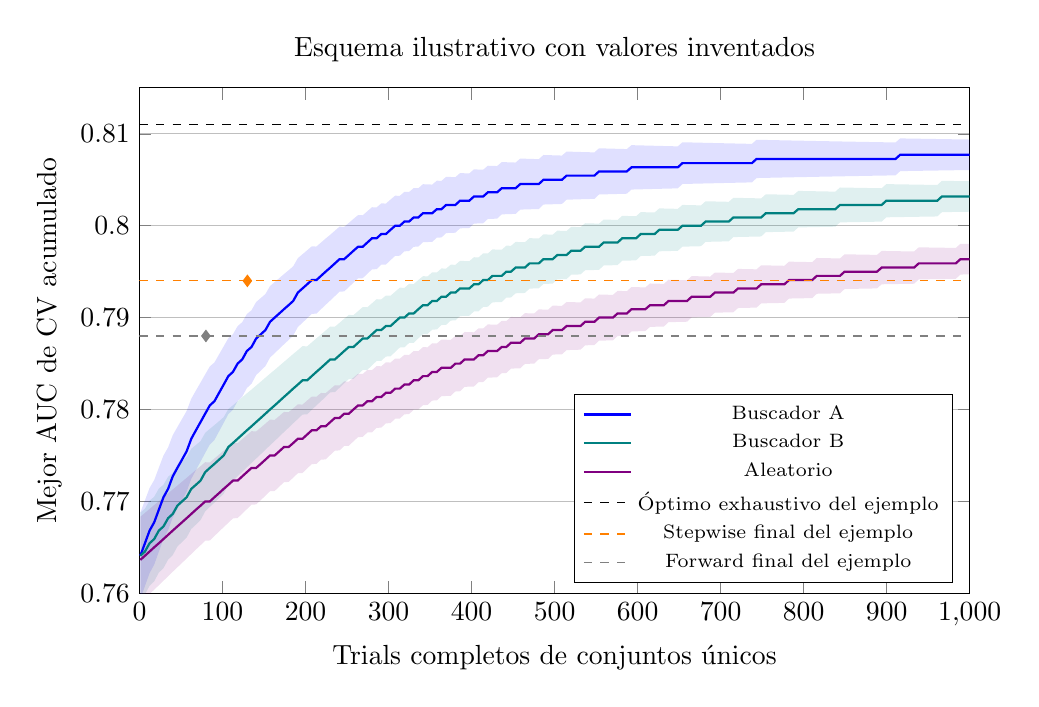
\begin{tikzpicture}
\begin{axis}[
width=\linewidth,height=8cm,
xmin=0,xmax=1000,ymin=0.760,ymax=0.815,
xlabel={Trials completos de conjuntos únicos},
ylabel={Mejor AUC de CV acumulado},
title={Esquema ilustrativo con valores inventados},
legend style={font=\scriptsize,at={(0.98,0.02)},anchor=south east},
ymajorgrids=true,scaled y ticks=false,
]
\addplot[name path=upper0,draw=none,forget plot,domain=1:1000,samples=180] {floor(2200*(0.764+(0.808-0.764)*(1-exp(-x/180))))/2200+(0.004*exp(-x/700)+0.0007)};
\addplot[name path=lower0,draw=none,forget plot,domain=1:1000,samples=180] {floor(2200*(0.764+(0.808-0.764)*(1-exp(-x/180))))/2200-(0.004*exp(-x/700)+0.0007)};
\addplot[blue,opacity=0.12,forget plot] fill between[of=upper0 and lower0];
\addplot[blue,thick,domain=1:1000,samples=180] {floor(2200*(0.764+(0.808-0.764)*(1-exp(-x/180))))/2200};
\addlegendentry{Buscador A}
\addplot[name path=upper1,draw=none,forget plot,domain=1:1000,samples=180] {floor(2200*(0.764+(0.805-0.764)*(1-exp(-x/310))))/2200+(0.004*exp(-x/700)+0.0007)};
\addplot[name path=lower1,draw=none,forget plot,domain=1:1000,samples=180] {floor(2200*(0.764+(0.805-0.764)*(1-exp(-x/310))))/2200-(0.004*exp(-x/700)+0.0007)};
\addplot[teal,opacity=0.12,forget plot] fill between[of=upper1 and lower1];
\addplot[teal,thick,domain=1:1000,samples=180] {floor(2200*(0.764+(0.805-0.764)*(1-exp(-x/310))))/2200};
\addlegendentry{Buscador B}
\addplot[name path=upper2,draw=none,forget plot,domain=1:1000,samples=180] {floor(2200*(0.764+(0.8-0.764)*(1-exp(-x/430))))/2200+(0.004*exp(-x/700)+0.0007)};
\addplot[name path=lower2,draw=none,forget plot,domain=1:1000,samples=180] {floor(2200*(0.764+(0.8-0.764)*(1-exp(-x/430))))/2200-(0.004*exp(-x/700)+0.0007)};
\addplot[violet,opacity=0.12,forget plot] fill between[of=upper2 and lower2];
\addplot[violet,thick,domain=1:1000,samples=180] {floor(2200*(0.764+(0.8-0.764)*(1-exp(-x/430))))/2200};
\addlegendentry{Aleatorio}
\addplot[black,dashed] coordinates {(0,0.811) (1000,0.811)};
\addlegendentry{Óptimo exhaustivo del ejemplo}
\addplot[orange,dashed] coordinates {(0,0.794) (1000,0.794)};
\addlegendentry{Stepwise final del ejemplo}
\addplot[gray,dashed] coordinates {(0,0.788) (1000,0.788)};
\addlegendentry{Forward final del ejemplo}
\addplot[orange,only marks,mark=diamond*,forget plot] coordinates {(130,0.794)};
\addplot[gray,only marks,mark=diamond*,forget plot] coordinates {(80,0.788)};
\end{axis}
\end{tikzpicture}
\caption{Esquema ilustrativo del gráfico propuesto. Todos los valores son inventados.}
\label{fig:convergencia}
\end{figure}

\textbf{Figura 1.} Esquema con valores inventados exclusivamente para mostrar el diseño. No representa ejecuciones, intervalos reales ni un pronóstico de rendimiento. En el estudio se reemplazarán todas las curvas y referencias por resultados del evaluador común. La separación gráfica entre algoritmos no anticipa cuál será superior.

\subsection{Brecha y tiempo hasta una solución cercana}\label{sec:11.2}

La brecha absoluta al óptimo será:

\[
r_{a,r}(t)=J^*-b_{a,r}(t).
\]

Para una tolerancia \(\epsilon\) se definirá el primer ensayo que alcanza esa cercanía:

\[
T_{\epsilon,a,r}=\min\{t:r_{a,r}(t)\leq\epsilon\}.
\]

Se propondrán tolerancias absolutas de AUC de 0,005, 0,002 y 0,001. Las ejecuciones que no alcancen la tolerancia antes del presupuesto quedarán censuradas; no se eliminarán ni se calculará una media usando solo las exitosas. Se reportará tasa de éxito y distribución del tiempo hasta el objetivo.

Se resumirá además la brecha media a lo largo del presupuesto:

\[
R_B=\frac{1}{B}\sum_{t=1}^{B}r_{a,r}(t).
\]

Un menor valor premia encontrar buenas soluciones temprano y mantenerlas. Este indicador se denominará brecha integrada, evitando confundirlo con el AUC predictivo. Si un método termina antes, su mejor valor podrá mantenerse para el gráfico hasta B, señalando explícitamente que dejó de evaluar.

\subsection{Resultados adicionales que deberán publicarse}\label{sec:11.3}

Se incluirán la proporción del espacio evaluada, candidatos rechazados por causa, diversidad de población y capacidad prequential del sustituto. Para cada solución final se reportarán AUC externo, KS, calibración, número de variables y frecuencia de selección. También se estudiará la distancia al óptimo en desempeño sin exigir recuperar exactamente sus variables: puede haber muchos subconjuntos casi equivalentes.

Un resultado donde SEF llegue antes al óptimo de CV, pero no mejore AUC externo, seguirá demostrando eficiencia de optimización si la medición es correcta; no demostrará una mejor scorecard predictiva. Un resultado de igual calidad y menor tiempo también puede ser útil. Ambos tipos de conclusión deben distinguirse.

\section{Ablaciones y análisis de sensibilidad}\label{sec:12}

Las ablaciones obligatorias retirarán por separado sustituto, búsqueda local, movimientos dobles, reinicios e inicialización guiada. Se comparará el tratamiento de restricciones por generación y reparación frente a rechazo simple. Cada comparación conservará presupuesto, evaluador, tareas y semillas comunes cuando sea posible.

Se estudiará sensibilidad a tamaño de población, proporción aleatoria, cardinalidad, umbral IV y densidad del grafo de conflictos. Cambiar IV o correlación redefine el espacio admisible: su efecto no se interpretará como una mejora del optimizador. Estas variaciones serán experimentos de especificación del problema.

La comparación AUC versus KS repetirá búsquedas con cada objetivo y examinará estabilidad del ranking de candidatos sobre remuestras, desempeño externo y sensibilidad a eventos escasos. Para evaluar variabilidad de la métrica aislada se usarán predicciones de candidatos fijos; para evaluar estabilidad del procedimiento se repetirá toda la selección. Son experimentos distintos.

Una extensión posterior podrá usar baja fidelidad mediante menos observaciones o folds y promoción a evaluación completa. Requerirá medir conservación de ranking y contabilizar recursos equivalentes. No se mezclará esa extensión con la comparación primaria hasta disponer de una referencia exacta estable.

\section{Límites y criterios de interpretación}\label{sec:13}

Una restricción de familia protege una definición de negocio, pero puede excluir señal complementaria. Un IV alto no garantiza aporte incremental y uno bajo no demuestra inutilidad condicional. Correlación y VIF controlan propiedades estadísticas concretas; no prueban causalidad, ausencia de fuga ni coherencia económica.

La optimización puede explotar ruido de validación, incluso con un objetivo razonable y miles de evaluaciones reproducibles. El sustituto puede concentrar la búsqueda prematuramente en una región incorrecta. La diversidad, las propuestas aleatorias y los reinicios son mecanismos de mitigación que deben probarse, no garantías.

Un máximo de CV muy preciso puede coexistir con incertidumbre considerable sobre desempeño futuro. Los p valores convencionales de una logística después de una búsqueda extensa no constituyen inferencia selectiva válida por el solo hecho de tener signos coherentes y VIF bajo. No se usarán para justificar retrospectivamente la optimalidad de las variables elegidas.

La implementación en un banco requerirá revisar su uso concreto frente a las políticas internas y la normativa aplicable. La Recopilación Actualizada de Normas de la CMF será una fuente primaria para esa revisión \cite{ref14}. Este documento no atribuye exigencias normativas a IV, correlación, VIF, algoritmo de búsqueda o tolerancias propuestas, ni afirma que el selector implique aprobación regulatoria.

\section{Plan de desarrollo posterior}\label{sec:14}

La primera entrega deberá ser el contrato del problema: definición del target, unidad de observación, fechas de disponibilidad, catálogo de familias, reglas y protocolo de validación. Antes de construir un optimizador, se implementará el evaluador común y se comprobará manualmente sobre conjuntos pequeños con resultados verificables.

La segunda entrega será un benchmark exhaustivo pequeño con búsqueda aleatoria, forward e intercambios. Permitirá verificar la caché, los conteos, la factibilidad y la reproducción de curvas. La tercera incorporará el genético por familias; solo después se añadirán mejora local y sustituto, conservando versiones separadas para ablación.

La cuarta entrega será el estudio de generalización en datos públicos y cortes históricos autorizados. La decisión de adoptar componentes se basará en mejora repetida y costo total. Si el sustituto no aporta, se mantendrá la versión genética o local más simple. Si un método clásico alcanza consistentemente soluciones equivalentes con menos recursos, esa será una conclusión válida del estudio.

El resultado esperado de la investigación será un procedimiento reproducible para encontrar y justificar conjuntos factibles con presupuesto limitado. La ambición técnica es mejorar la selección de scorecards mediante evidencia comparativa; la superioridad quedará abierta hasta completar los experimentos.


\begin{thebibliography}{99}
\bibitem{ref1} Lappas, P. Z. y Yannacopoulos, A. N. (2021). A machine learning approach combining expert knowledge with genetic algorithms in feature selection for credit risk assessment. Applied Soft Computing, 107, 107391. \url{https://doi.org/10.1016/j.asoc.2021.107391}

\bibitem{ref2} Baptista, R. y Poloczek, M. (2018). Bayesian Optimization of Combinatorial Structures. ICML, PMLR 80, 462--471. \url{https://proceedings.mlr.press/v80/baptista18a.html}

\bibitem{ref3} Wan, X., Nguyen, V., Ha, H., Ru, B., Lu, C. y Osborne, M. A. (2021). Think Global and Act Local Bayesian Optimisation over High Dimensional Categorical and Mixed Search Spaces. ICML, PMLR 139, 10663--10674. \url{https://proceedings.mlr.press/v139/wan21b.html}

\bibitem{ref4} Altarabichi, M. G., Nowaczyk, S., Pashami, S. y Sheikholharam Mashhadi, P. (2021). Surrogate Assisted Genetic Algorithm for Wrapper Feature Selection. Manuscrito accesible en arXiv. \url{https://arxiv.org/abs/2111.09074}

\bibitem{ref5} Altarabichi, M. G., Nowaczyk, S., Pashami, S. y Sheikholharam Mashhadi, P. (2023). Fast Genetic Algorithm for feature selection A qualitative approximation approach. Expert Systems with Applications, 211, 118528. Manuscrito depositado en 2024. \url{https://doi.org/10.1016/j.eswa.2022.118528} ; \url{https://arxiv.org/abs/2404.03996}

\bibitem{ref6} Cawley, G. C. y Talbot, N. L. C. (2010). On Over fitting in Model Selection and Subsequent Selection Bias in Performance Evaluation. Journal of Machine Learning Research, 11, 2079--2107. \url{https://jmlr.org/papers/v11/cawley10a.html}

\bibitem{ref7} Nogueira, S., Sechidis, K. y Brown, G. (2018). On the Stability of Feature Selection Algorithms. Journal of Machine Learning Research, 18(174), 1--54. \url{https://jmlr.org/papers/v18/17-514.html}

\bibitem{ref8} Deb, K. (2000). An efficient constraint handling method for genetic algorithms. Computer Methods in Applied Mechanics and Engineering, 186, 311--338. \url{https://doi.org/10.1016/S0045-7825(99)00389-8}

\bibitem{ref9} Hanley, J. A. y McNeil, B. J. (1982). The meaning and use of the area under a receiver operating characteristic ROC curve. Radiology, 143(1), 29--36. \url{https://doi.org/10.1148/radiology.143.1.7063747}

\bibitem{ref10} Optuna. Documentación oficial de TPESampler. Consulta del 22 de septiembre de 2026. \url{https://optuna.readthedocs.io/en/stable/reference/samplers/generated/optuna.samplers.TPESampler.html}

\bibitem{ref11} Navas Palencia, G. OptBinning. Documentación oficial de binning y scorecards. Referencia técnica candidata para implementación, no dependencia decidida. \url{https://gnpalencia.org/optbinning/scorecard.html}

\bibitem{ref12} Yeh, I. Default of Credit Card Clients. UCI Machine Learning Repository. \url{https://doi.org/10.24432/C55S3H}

\bibitem{ref13} UCI Machine Learning Repository. South German Credit. \url{https://archive.ics.uci.edu/dataset/522/south+german+credit}

\bibitem{ref14} Comisión para el Mercado Financiero. Recopilación Actualizada de Normas de Bancos. Catálogo oficial consultado el 22 de septiembre de 2026. \url{https://www.cmfchile.cl/portal/normativa/624/w4-propertyvalue-49163.html}
\end{thebibliography}
\end{document}
